\documentclass[10pt,aspectratio=169]{beamer}
\usetheme{Madrid}
\usecolortheme{whale}
\usepackage[utf8]{inputenc}
\usepackage[T1]{fontenc}
\usepackage[brazil]{babel}
\usepackage{booktabs}
\usepackage{graphicx}

\setbeamertemplate{navigation symbols}{}
\setbeamertemplate{blocks}[rounded][shadow=true]

\title[Otimização de Matmul com OpenMP]{Otimização de Multiplicação de Matrizes com OpenMP:\\vetorização, granularidade e padrão de acesso à memória}
\subtitle{Trabalho Final --- Software de Alto Desempenho (INF01094)}
\author{João Vitor do Amaral Spolavore}
\institute{Instituto de Informática --- UFRGS}
\date{2026/1}

\begin{document}

% ---------------------------------------------------------------- 1. titulo
\begin{frame}
  \titlepage
\end{frame}

% ---------------------------------------------------------------- 2. problema + ambiente
\begin{frame}{Problema, aplicação e ambiente}
  \begin{columns}[T]
    \column{0.52\textwidth}
      \textbf{Problema}
      \begin{itemize}
        \item Multiplicação de matrizes densas $C = A \times B$, dupla precisão, $N = 1024$;
        \item $2N^3 \approx 2{,}15$ GFLOP por execução; 24 MiB de dados;
        \item núcleo de álgebra linear, simulação e ML; reuso de dados e paralelismo abundante.
      \end{itemize}
      \begin{block}{Pergunta da investigação}
        Quais intervenções OpenMP produzem ganho real, quais não produzem, e \emph{por quê}?
      \end{block}
    \column{0.44\textwidth}
      \textbf{Ambiente: PCAD/UFRGS, nó hype5}
      \begin{itemize}
        \item 2$\times$ Xeon E5-2650 v3 (Haswell): \textbf{20 cores / 40 threads HT, 2 sockets NUMA};
        \item 128 GB DDR4; L3 25 MiB/socket;
        \item governor de frequência fixo em \texttt{performance}.
      \end{itemize}
  \end{columns}
\end{frame}

% ---------------------------------------------------------------- 3. baseline
\begin{frame}[fragile]{Baseline (v0) e metodologia de medição}
  \begin{columns}[T]
    \column{0.46\textwidth}
      \textbf{v0: laços i-j-k canônicos}
\begin{semiverbatim}\small
for (i = 0; i < n; i++)
  for (j = 0; j < n; j++) \{
    double sum = 0.0;
    for (k = 0; k < n; k++)
      sum += A[i*n+k] * B[k*n+j];
    C[i*n+j] = sum;
  \}
\end{semiverbatim}
      \textbf{Baseline: 2,298 s} ($\sigma$ = 0,0003)
    \column{0.50\textwidth}
      \textbf{Metodologia}
      \begin{itemize}
        \item \textbf{sem profiler}: tempo medido com \texttt{omp\_get\_wtime()} em volta do kernel;
        \item 1 warm-up não medido + \textbf{5 repetições}; mediana $\pm$ desvio ($<1\%$);
        \item threads fixadas nos cores físicos:\\ \texttt{OMP\_PROC\_BIND=close}, \texttt{OMP\_PLACES=cores};
        \item mesmas entradas em todas as versões;
        \item \textbf{validação}: comparação elemento a elemento com a v0 --- diferença \textbf{zero} nas 4 versões.
      \end{itemize}
  \end{columns}
\end{frame}

% ---------------------------------------------------------------- 4. diagnostico
\begin{frame}{Diagnóstico do gargalo}
  \begin{itemize}
    \item Pico teórico do nó $\approx$ 736 GFLOP/s; a v0 atinge \textbf{0,94 GFLOP/s $\approx$ 0,1\%} $\rightarrow$ o gargalo \textbf{não} é processamento.
    \item Laço interno lê \texttt{B[k*n+j]} com \textbf{stride de 8 KiB}: cada iteração toca uma linha de cache nova e usa só 1 dos 8 doubles trazidos.
    \item Sintoma do mapa da disciplina: \emph{tempo dominado por memória / acessos com stride}.
  \end{itemize}
\end{frame}

% ---------------------------------------------------------------- 5. v1
\begin{frame}[fragile]{v1 --- \texttt{omp simd} no laço interno (sem ganho)}
  \begin{columns}[T]
    \column{0.5\textwidth}
\begin{semiverbatim}\small
double sum = 0.0;
#pragma omp simd reduction(+:sum)
for (k = 0; k < n; k++)
  sum += A[i*n+k] * B[k*n+j];
\end{semiverbatim}
      \begin{itemize}
        \item \textbf{Hipótese:} SIMD processa 4 doubles por instrução (AVX2) $\rightarrow$ $\sim$4$\times$.
      \end{itemize}
    \column{0.46\textwidth}
      \begin{itemize}
        \item O compilador \textbf{vetoriza de fato}, mas monta os vetores de \texttt{B} com cargas escalares --- o acesso tem stride;
        \item o tráfego de memória por iteração \textbf{não muda}.
      \end{itemize}
      \begin{alertblock}{Resultado medido}
        2,388 s $\rightarrow$ \textbf{0,96$\times$} (leve piora)
      \end{alertblock}
  \end{columns}
\end{frame}

% ---------------------------------------------------------------- 6. v2 e v3
\begin{frame}[fragile]{v2 e v3 --- a MESMA técnica, granularidades opostas}
  \begin{columns}[T]
    \column{0.48\textwidth}
      \textbf{v2: laço externo (grossa)}
\begin{semiverbatim}\small
#pragma omp parallel for \\
        schedule(static)
for (i = 0; i < n; i++)
  ... /* corpo igual ao da v0 */
\end{semiverbatim}
      \begin{itemize}
        \item 1 região paralela; $N/p$ linhas por thread, sem sincronização interna.
      \end{itemize}
    \column{0.48\textwidth}
      \textbf{v3: laço interno (fina)}
\begin{semiverbatim}\small
for (i ...) for (j ...) \{
#pragma omp parallel for \\
        reduction(+:sum)
  for (k = 0; k < n; k++) ...
\}
\end{semiverbatim}
      \begin{itemize}
        \item Região paralela criada $N^2 \approx 10^6$ vezes; reduction + \textbf{barreira entre 2 sockets} a cada vez.
      \end{itemize}
  \end{columns}
\end{frame}

% ---------------------------------------------------------------- 7. resultados v2 v3
\begin{frame}{v2 e v3 --- resultados (20 threads)}
  \vfill
  \begin{columns}[T]
    \column{0.44\textwidth}
      \begin{block}{v2 --- laço externo (grossa)}
        \centering
        {\Large \textbf{0,132 s $\rightarrow$ 17,5$\times$}}
      \end{block}
    \column{0.44\textwidth}
      \begin{alertblock}{v3 --- laço interno (fina)}
        \centering
        {\Large \textbf{10,193 s $\rightarrow$ 0,23$\times$}}
      \end{alertblock}
  \end{columns}
  \vfill
  \centering
  Baseline v0 (1 thread): \textbf{2,298 s} --- com os mesmos 20 cores, a v3 ficou \alert{4,4$\times$ mais lenta} que o sequencial.
  \vfill
\end{frame}

% ---------------------------------------------------------------- 8. escalabilidade
\begin{frame}{Escalabilidade da v2}
  \begin{columns}[T]
    \column{0.5\textwidth}
      \centering
      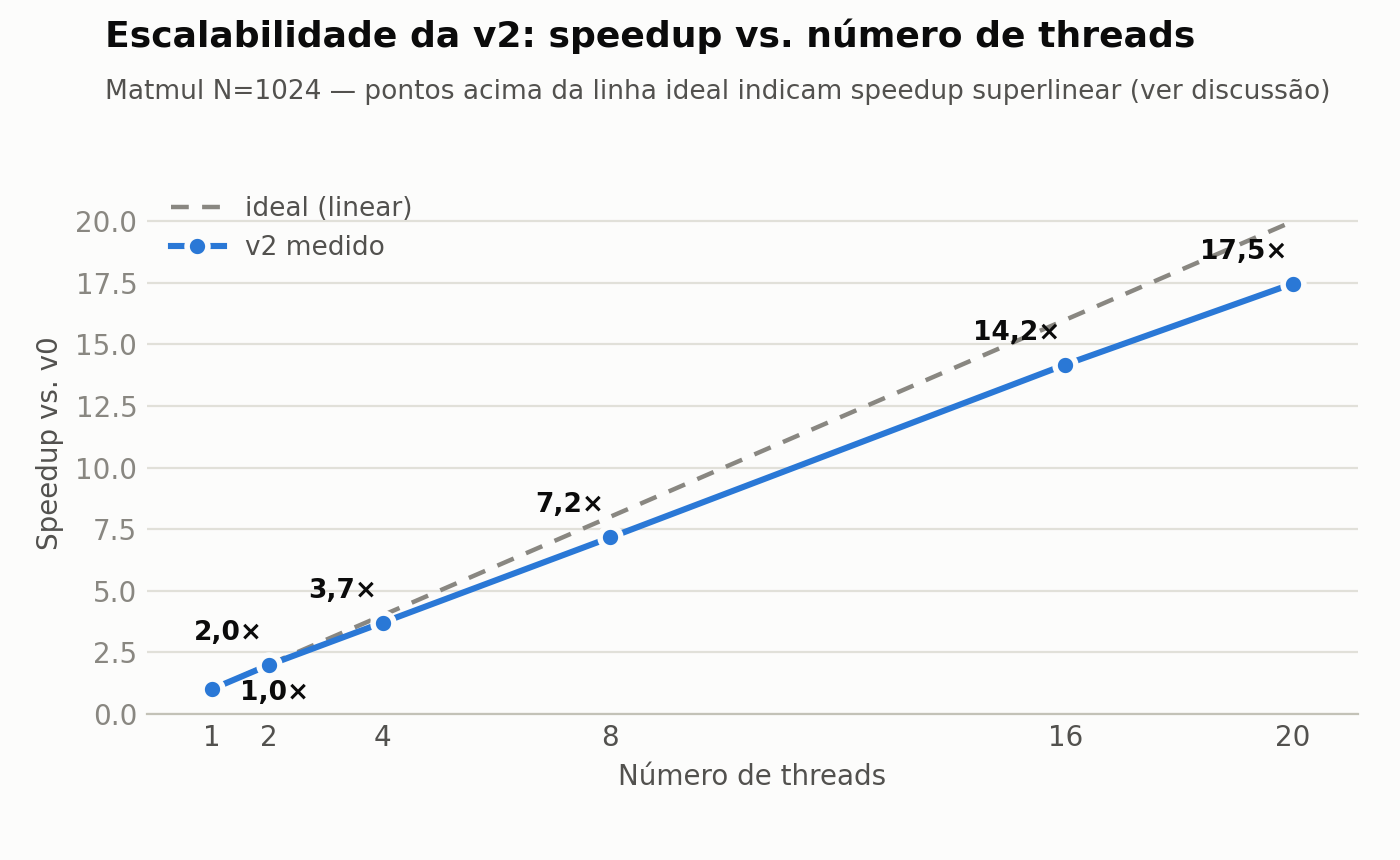
\includegraphics[width=\textwidth]{../results-hype/escalabilidade_v2.png}
    \column{0.5\textwidth}
      \centering
      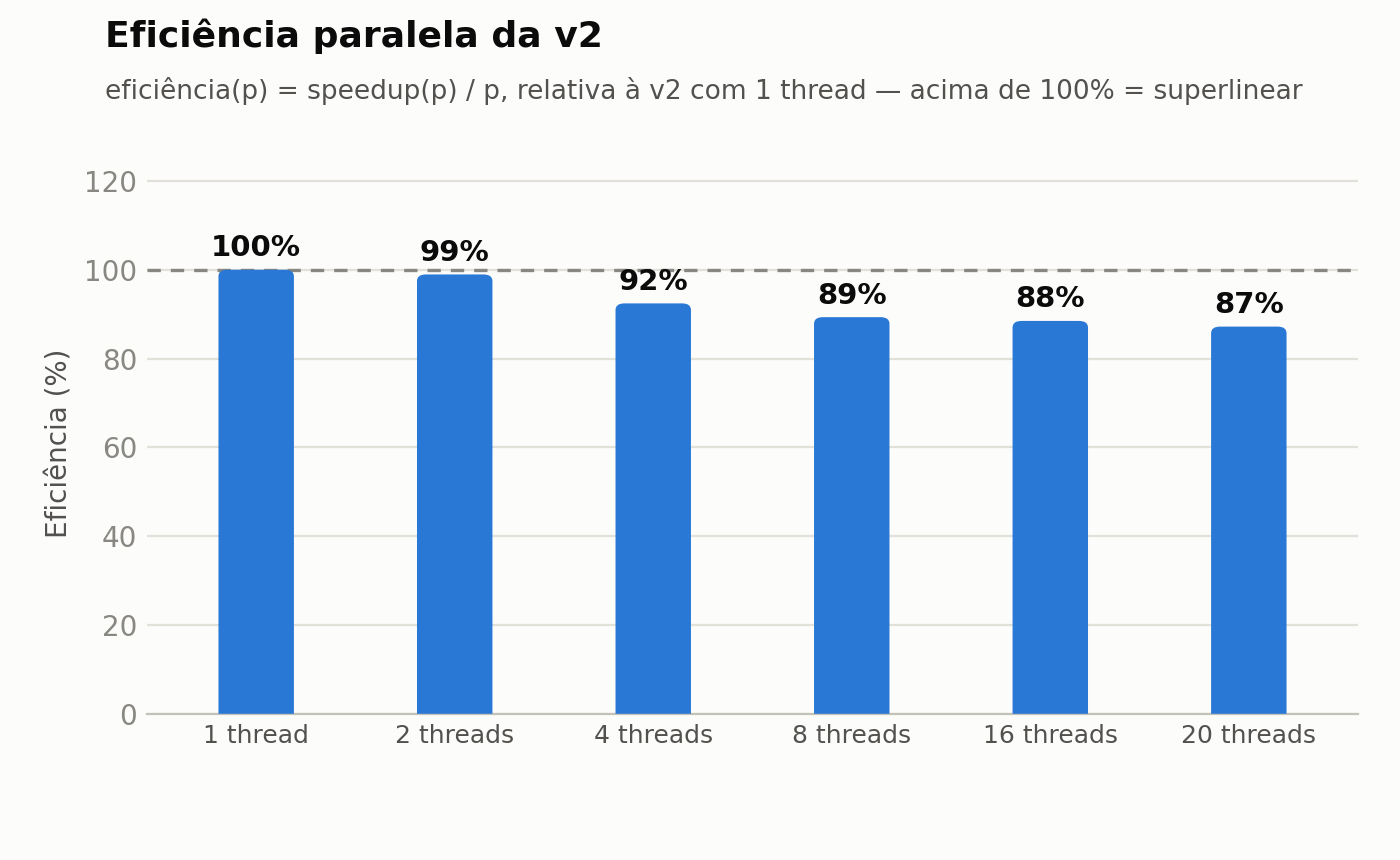
\includegraphics[width=\textwidth]{../results-hype/eficiencia_v2.png}
  \end{columns}
  \vfill
  \centering
  Quase linear até 20 threads (99\% $\rightarrow$ 87\%); a queda gradual acompanha a fronteira NUMA.
\end{frame}

% ---------------------------------------------------------------- 7. v4
\begin{frame}[fragile]{v4 --- troca de laços i-k-j (ataca a causa raiz)}
  \begin{columns}[T]
    \column{0.5\textwidth}
\begin{semiverbatim}\small
#pragma omp parallel for \\
        schedule(static)
for (i = 0; i < n; i++) \{
  for (j ...) C[i*n+j] = 0.0;
  for (k = 0; k < n; k++) \{
    const double a = A[i*n+k];
    for (j = 0; j < n; j++)
      C[i*n+j] += a * B[k*n+j];
  \}
\}
\end{semiverbatim}
    \column{0.46\textwidth}
      \begin{itemize}
        \item Laço interno percorre \texttt{B} e \texttt{C} com \textbf{stride 1}: vetorização efetiva, prefetch sequencial, linha de cache usada por inteiro;
        \item soma na mesma ordem de $k$ $\rightarrow$ resultado \textbf{bit a bit idêntico} ao da v0;
        \item combina a correção do padrão de acesso com o paralelismo da v2.
      \end{itemize}
  \end{columns}
\end{frame}

% ---------------------------------------------------------------- 8. resultados
\begin{frame}{Resultados (hype, $N=1024$, mediana de 5 repetições)}
  \begin{table}
    \centering
    \begin{tabular}{llrrrr}
      \toprule
      Versão & Configuração & Tempo & Speedup & GFLOP/s & Efic.\\
      \midrule
      v0 & sequencial                    & 2,298 s  & 1,00$\times$          & 0,94 & --- \\
      v1 & \texttt{omp simd}, sequencial & 2,388 s  & \textbf{0,96$\times$} & 0,90 & --- \\
      v3 & paralelo interno, 20 threads  & 10,193 s & \alert{\textbf{0,23$\times$}} & 0,21 & 1\% \\
      v2 & paralelo externo, 20 threads  & 0,132 s  & 17,47$\times$         & 16,3 & 87\% \\
      v4 & i-k-j (troca de laços), 1 thread & 0,289 s & 7,9$\times$ & 7,4 & --- \\
      v4 & i-k-j + paralelo, 20 threads  & \textbf{0,017 s} & \textbf{132$\times$} & \textbf{123,5} & 83\% \\
      \bottomrule
    \end{tabular}
  \end{table}
\end{frame}

% ---------------------------------------------------------------- 9. grafico speedup
\begin{frame}{Speedup por versão}
  \centering
  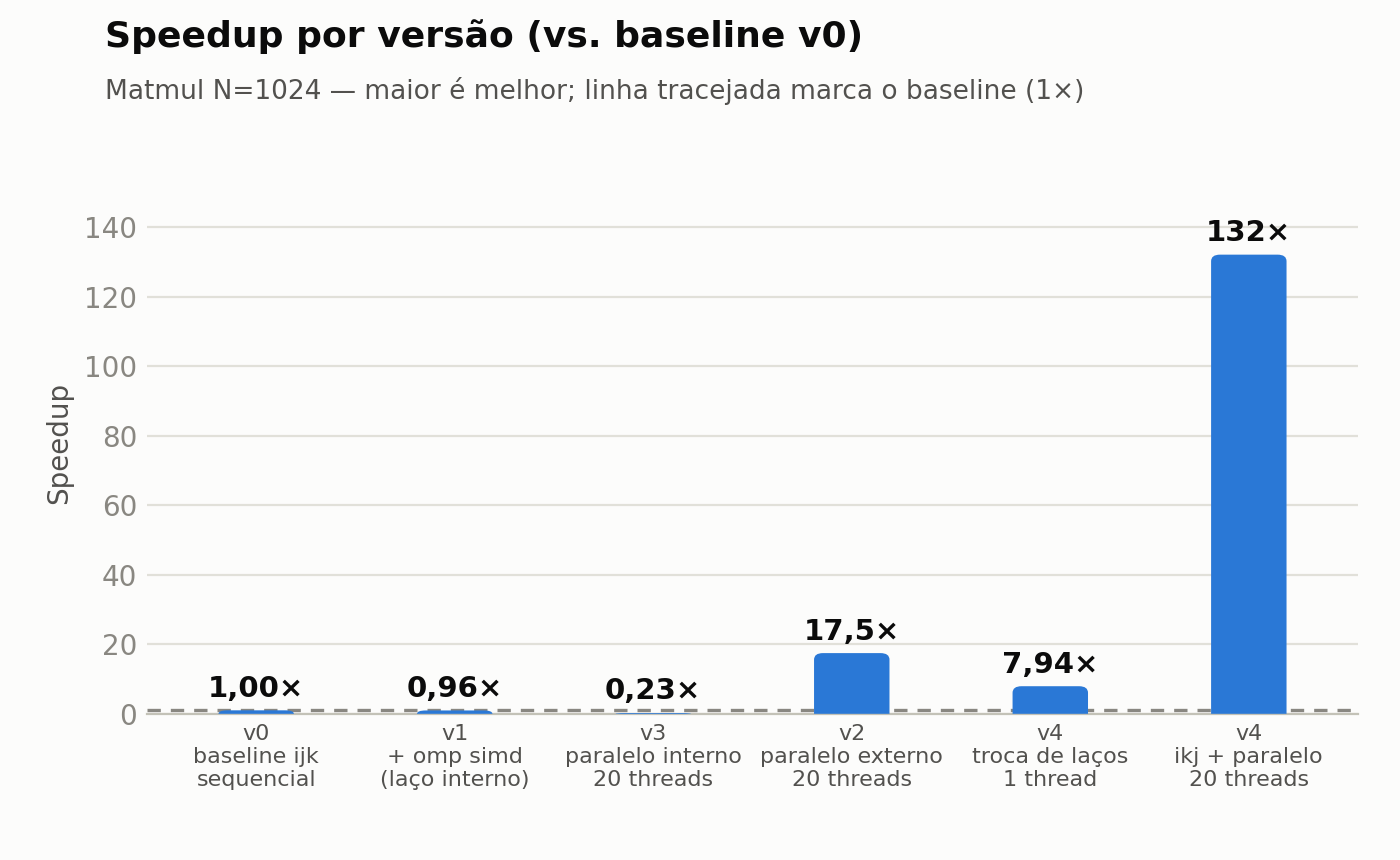
\includegraphics[height=0.78\textheight]{../results-hype/speedup_por_versao.png}
\end{frame}

% ---------------------------------------------------------------- 12. discussao
\begin{frame}{Discussão: por que cada resultado aconteceu}
  \begin{itemize}
    \item \textbf{v1 (0,96$\times$):} SIMD multiplica a capacidade de cálculo, mas o tempo é gasto esperando memória. \emph{Uma técnica só é boa otimização quando resolve o gargalo dominante.}
    \item \textbf{v3 (0,23$\times$):} $10^6$ regiões paralelas $\Rightarrow$ fork/join + barreiras \textbf{atravessando 2 sockets NUMA} custam mais que o trabalho útil.
    \item \textbf{v2 (17,5$\times$, 87\%):} granularidade grossa escala quase linear; a eficiência cai suavemente ao ocupar o segundo socket (acessos NUMA remotos).
    \item \textbf{v4 (132$\times$):} o par v1/v4 fecha a prova --- as mesmas unidades SIMD rendem 0,96$\times$ com stride e 7,9$\times$ (1 thread) com acesso corrigido; com 20 threads, 123,5 GFLOP/s.
  \end{itemize}
\end{frame}

% ---------------------------------------------------------------- 12. agradecimento
\begin{frame}
  \centering
  {\Huge Obrigado}
\end{frame}

\end{document}
